\documentclass{article}

% Language setting
% Replace `english' with e.g. `spanish' to change the document language
\usepackage[english]{babel}
\usepackage{float}

% Set page size and margins
% Replace `letterpaper' with `a4paper' for UK/EU standard size

\usepackage[letterpaper,top=2cm,bottom=2cm,left=3cm,right=3cm,marginparwidth=1.75cm]{geometry}

% Useful packages
\usepackage{amsmath}
\usepackage{graphicx}
\usepackage{pgfplots}
\usepackage{filecontents}
\usepackage[colorlinks=true, allcolors=blue]{hyperref}
\usepackage{csvsimple}
\usepackage{natbib}
\usepackage{url}
\usepackage{booktabs}

\title{ELE670 - Assignement 1}
\author{Lunelli Riccardo,
Parola Riccardo,
Santini Gabriele}

\begin{document}
\maketitle

\begin{abstract}
\textit{Objective.} Classify patient pathology from EEG. 

\textit{Approach.} The classification task is performed using convolutional neural networks (CNNs), which have been widely used in computer vision and speech recognition to perform automatic feature extraction and classification but they also have successfully been applied to EEG signals. For this project we use EEGNet, a pretrained CNN model for EEG signals.

\textit{Main results.} Ma io che cazzo ne so...te posso cantà una canzone
\end{abstract}
\section{Introduction}
Working memory, a fundamental cognitive process, plays a pivotal role in our daily lives, serving as a cornerstone for various complex cognitive functions. Understanding the neural underpinnings of working memory has been a longstanding pursuit in neuroscience. To advance our comprehension of this cognitive process, we embark on a journey to delve into an electrophysiological dataset recorded from fifteen subjects during a verbal working memory task. 

In this paper, we undertake the task of comprehensively understanding and preprocessing this dataset. We will employ Python with MNE software for data visualization and preprocessing, allowing us to tap into the potential of this  dataset. Our report will encapsulate the entire process, starting with a detailed data description encompassing the study context, subject demographics, sampling approach, sampling rate, signal lengths, and trial epochs. Subsequently, we will elucidate our approach and implementation, presenting a flowchart of our methodology. Importantly, we will showcase the results obtained at each stage of our work, including preprocessing outcomes and any significant findings.

Throughout the paper, we will also discuss the achievements and implications of our work, shedding light on the insights gained from this dataset. Furthermore, we will candidly address the challenges and obstacles faced during the exploration and preprocessing of this dataset.


\section{Data descriptions}

The dataset \cite{ds004752:1.0.0} used for the assignment has been recorded from fifteen subjects during a verbal working memory task. Subjects were epilepsy patients undergoing intracranial monitoring for localization of epileptic seizures. Subjects performed a modified \href{https://rpadgett.butler.edu/nw221/sternberg_lab/index.html}{Sternberg task} in which the encoding of memory items, maintenance, and recall were temporally separated. Subject characteristics and information on sessions (set size, match/mismatch, correct/incorrect, response, response time for each trial) are also provided. This dataset enables the investigation of working memory by providing simultaneous scalp EEG and iEEG recordings, which can be used for connectivity analysis, alongside reconstructed beamforming EEG sources that can enable further cognitive analysis such as replay of memory items.

\begin{figure}
    \centering
    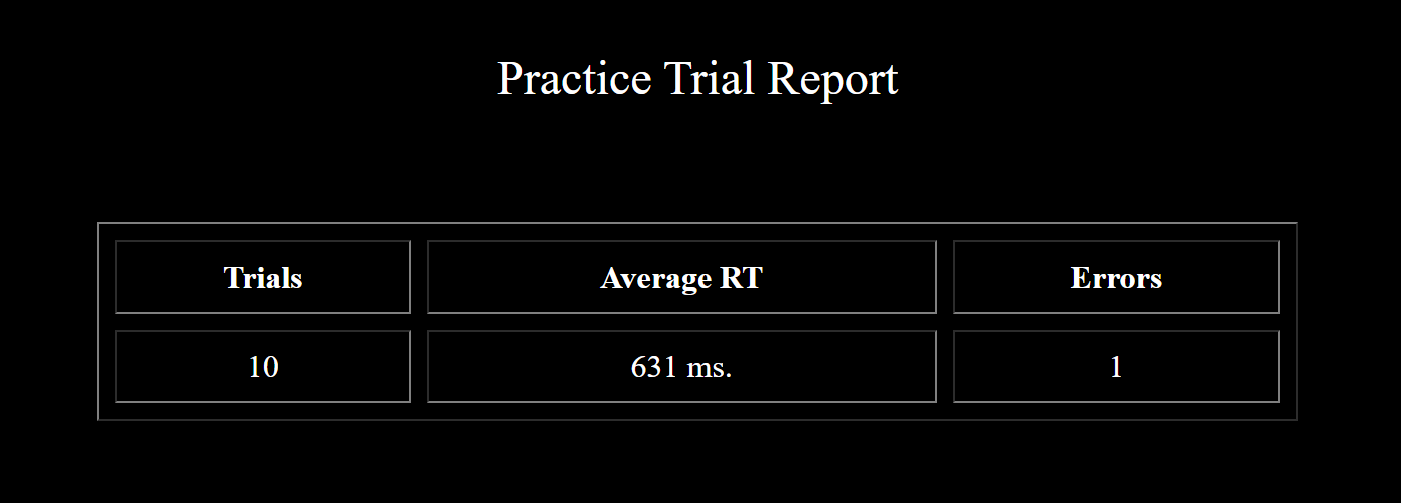
\includegraphics[width=0.5\linewidth]{img/test pappol.png}
    \caption{Our score at Sternberg Task}
    \label{fig:task}
\end{figure}

\newpage

\subsection{Subjects}

The dataset was recorded from fifteen subjects during a verbal working memory task. Each patient is identified using 3 different id system: usz, sciadv and elife. Additional recorded metadata includes the age of the participant at the time of the task, the self-reported gender of the participant, and the clinical diagnosis of the patient as shown in Figure \ref{fig:path_dist}. The shared characteristic among all patients is their confirmed diagnosis of focal epilepsy.
    
\begin{figure}[h]
  \centering
  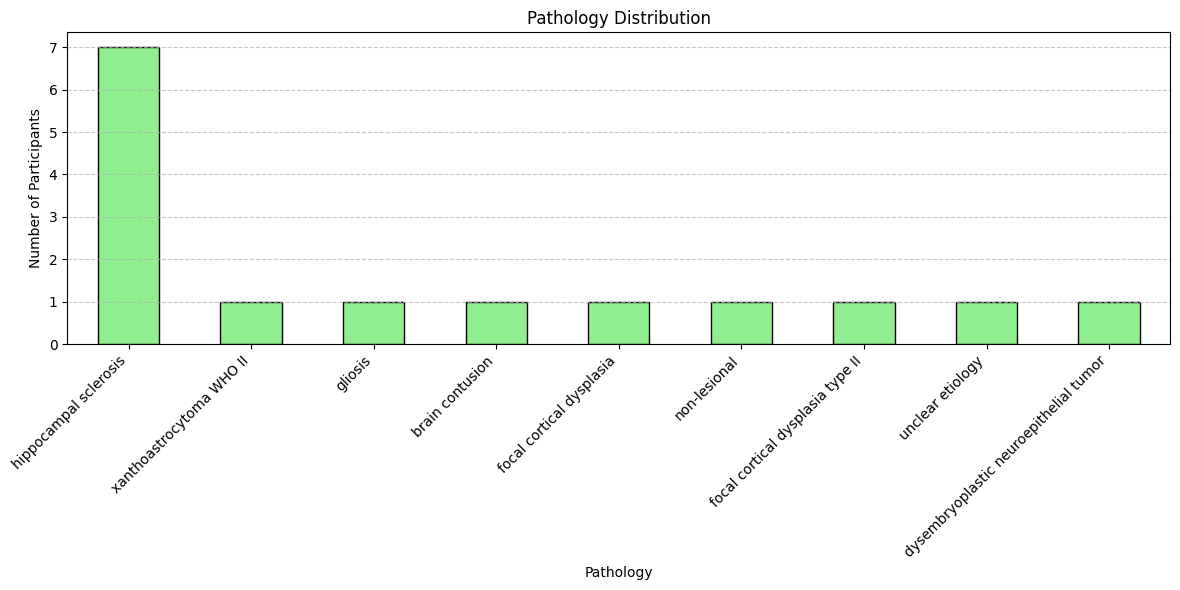
\includegraphics[width=0.8\textwidth]{img/pathology_dist.png}
  \caption{Pathology List Distribution}
  \label{fig:path_dist}
\end{figure}

Patients participated in multiple test sessions conducted on different days, Figure \ref{fig:session_distribution} visually represents the distribution of the number of sessions in which each patient participated.

\begin{figure}[ht]
  \centering
  \caption{Distribution of Number of Sessions}
  \begin{tikzpicture}
    \begin{axis}[
      ybar,
      bar width=0.5cm,
      width=12cm,
      height=6cm,
      xlabel={Patient},
      ylabel={Number of Sessions},
      ]
      \addplot table [x=Patient, y=Session, col sep=comma] {freq_dist.csv};
    \end{axis}
  \end{tikzpicture}
  \label{fig:session_distribution}
\end{figure}


\begin{figure}[h]
  \centering
  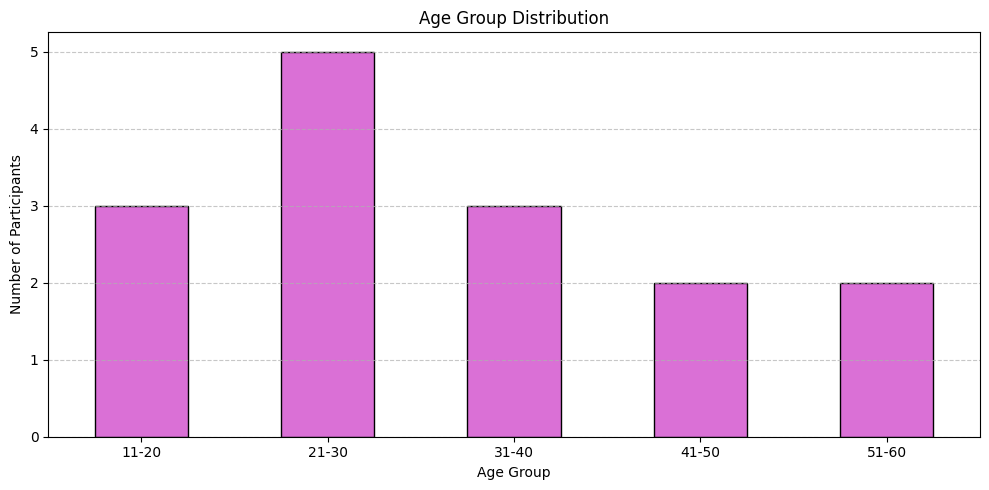
\includegraphics[width=0.7\textwidth]{img/Age_Group_Distribution.png}
  \caption{Age Group Distribution}
  \label{fig:Age}
\end{figure}

\begin{figure}[h]
  \centering
  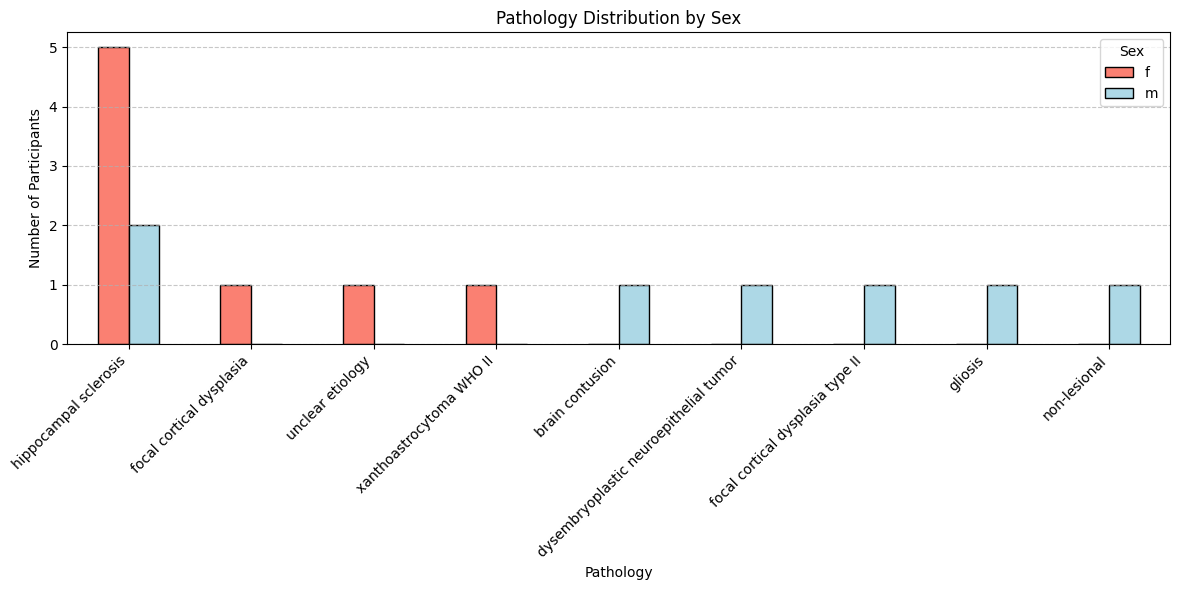
\includegraphics[width=0.8\textwidth]{img/pathology_dist_sex.png}
  \caption{Pathology Distribution by sex}
  \label{fig:sex}
\end{figure}

\subsection{Signal parameters}
The dataset includes simultaneously recorded scalp EEG with the 10-20 system, intracranial EEG (iEEG) recorded with depth electrodes, waveforms, and the MNI coordinates and anatomical labels of all intracranial electrodes. The dataset includes also reconstructed virtual sensor data that were created by performing LCMV beamforming on the EEG at specific brain regions including, temporal superior lobe, lateral prefrontal cortex, occipital cortex, posterior parietal cortex, and Broca. The data sampling frequency varied for different patients, with values of 200, 4000, or 4096 Hz, while the power line frequency was set at 50 Hz. Each subject participated in multiple working memory sessions, each comprising approximately 50 trials. Each trial included an encoding period of 2 seconds, a maintenance period of 3 seconds, and a subsequent probe letter presentation, during which participants indicated whether the probe was part of the memorized letter string. The EEG data was epoched with an epoch length of 8 seconds and was recorded using a high-pass filter with a cutoff frequency of 0.5 Hz and a low-pass filter with a cutoff frequency of 1000 Hz. 


    

\section{Pre-processing}
In this section, we will discuss the data pre-processing and its reasoning, motivations, and challenges. The dataset provided is very heterogeneous and part of the aim of this phase is to make it homogeneous and to create better conditions for learning.

\subsection{Data Loading}
The dataset follows the Brain Imaging Data Structure standard also called BIDS: Neuroimaging experiments generate complex data, often organized differently among researchers, causing confusion and wasted time. The Brain Imaging Data Structure (BIDS) provides a simple and widely accepted framework for organizing and sharing neuroimaging and behavioral data, promoting consistency and efficiency in research practices.

\begin{figure}[h]
  \centering
  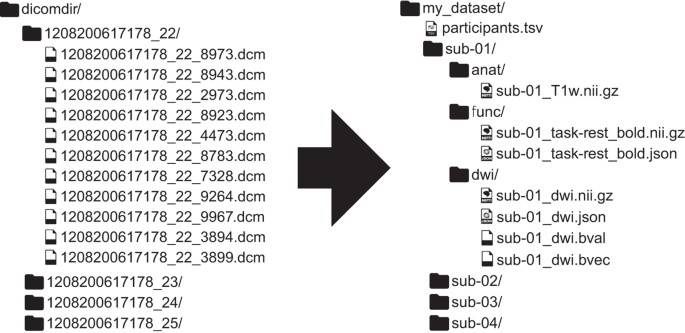
\includegraphics[width=0.6\textwidth]{img/bids_nature.jpg}
  \caption{BIDS standard structure}
  \label{fig:BIDS}
\end{figure}

This type of standard allows to use of tools such as the MNE library to easily import and apply some standard methods to the data.

\subsection{Frequency and Cannel Selection}
Not all patient data were collected the same way: for different patients in this dataset there might be different numbers of sensors or different frequencies of acquisition.
Most of the data were collected at 200hz and some were collected at a much higher frequency of 4000hz. We decided to convert all to 200hz since is the minimum possible to use.
The Nyquist-Shannon sampling theorem, a fundamental principle in signal processing, asserts that to accurately represent a signal, the sampling rate must be at least twice the frequency of the highest component in the signal. In the context of EEG data, this theorem holds significant implications.

Gamma waves, which are associated with higher cognitive functions, including memory and problem-solving, are typically found in the 30-100 Hz range of frequency. By adhering to the Nyquist criterion, we recognize that the sampling rate should be a minimum of twice the highest frequency component of interest. Therefore, in the case of gamma waves, using a 200 Hz sampling rate is justified. This choice allows us to accurately capture and represent the essential information contained within these high-frequency brain oscillations.

Not only was the frequency inconsistent across the dataset, but the number of channels or sensors used for EEG recordings also varied among different patients. This variation in the number of sensors adds another layer of complexity when standardizing the data for analysis.

We decided to use a consistent set of 8 channels for EEG sensors across all patient data. This decision was made for several reasons:
\begin{itemize}
    \item Data Consistency: By using the same set of 8 channels for all patients, we ensure data consistency, making it easier to compare and analyze EEG signals across different individuals.
    \item Reduced Dimensionality: While EEG systems can have a large number of channels (often 32 or more), using a reduced number of channels simplifies data processing and analysis.
    \item Consistency in Analysis: Researchers often focus their analyses on specific regions of the brain associated with the cognitive functions under investigation. By choosing a consistent set of 8 channels, we can ensure that the data we analyze are relevant to our research questions and hypotheses.
\end{itemize}


\subsubsection{Filtering and Artifact Removal}
Filtering is a very useful tool in data and signal analysis in our case we applied a low-pass filter with a lower cutoff frequency of 1 Hz to the EEG data. It removes low-frequency noise or drifts while preserving higher-frequency components.

Artifact Removal: Identify and remove artifacts from the EEG signal. Artifacts can include eye blinks, muscle movements, and electrical interference. This step may involve manual or automated artifact rejection techniques.

Epoching: Segment the continuous EEG data into shorter epochs or time windows. Each epoch typically corresponds to a specific event or stimulus in the experiment. This step allows you to analyze EEG responses to specific events.


\section{Flowchart of the method}

\begin{figure}[h]
  \centering
  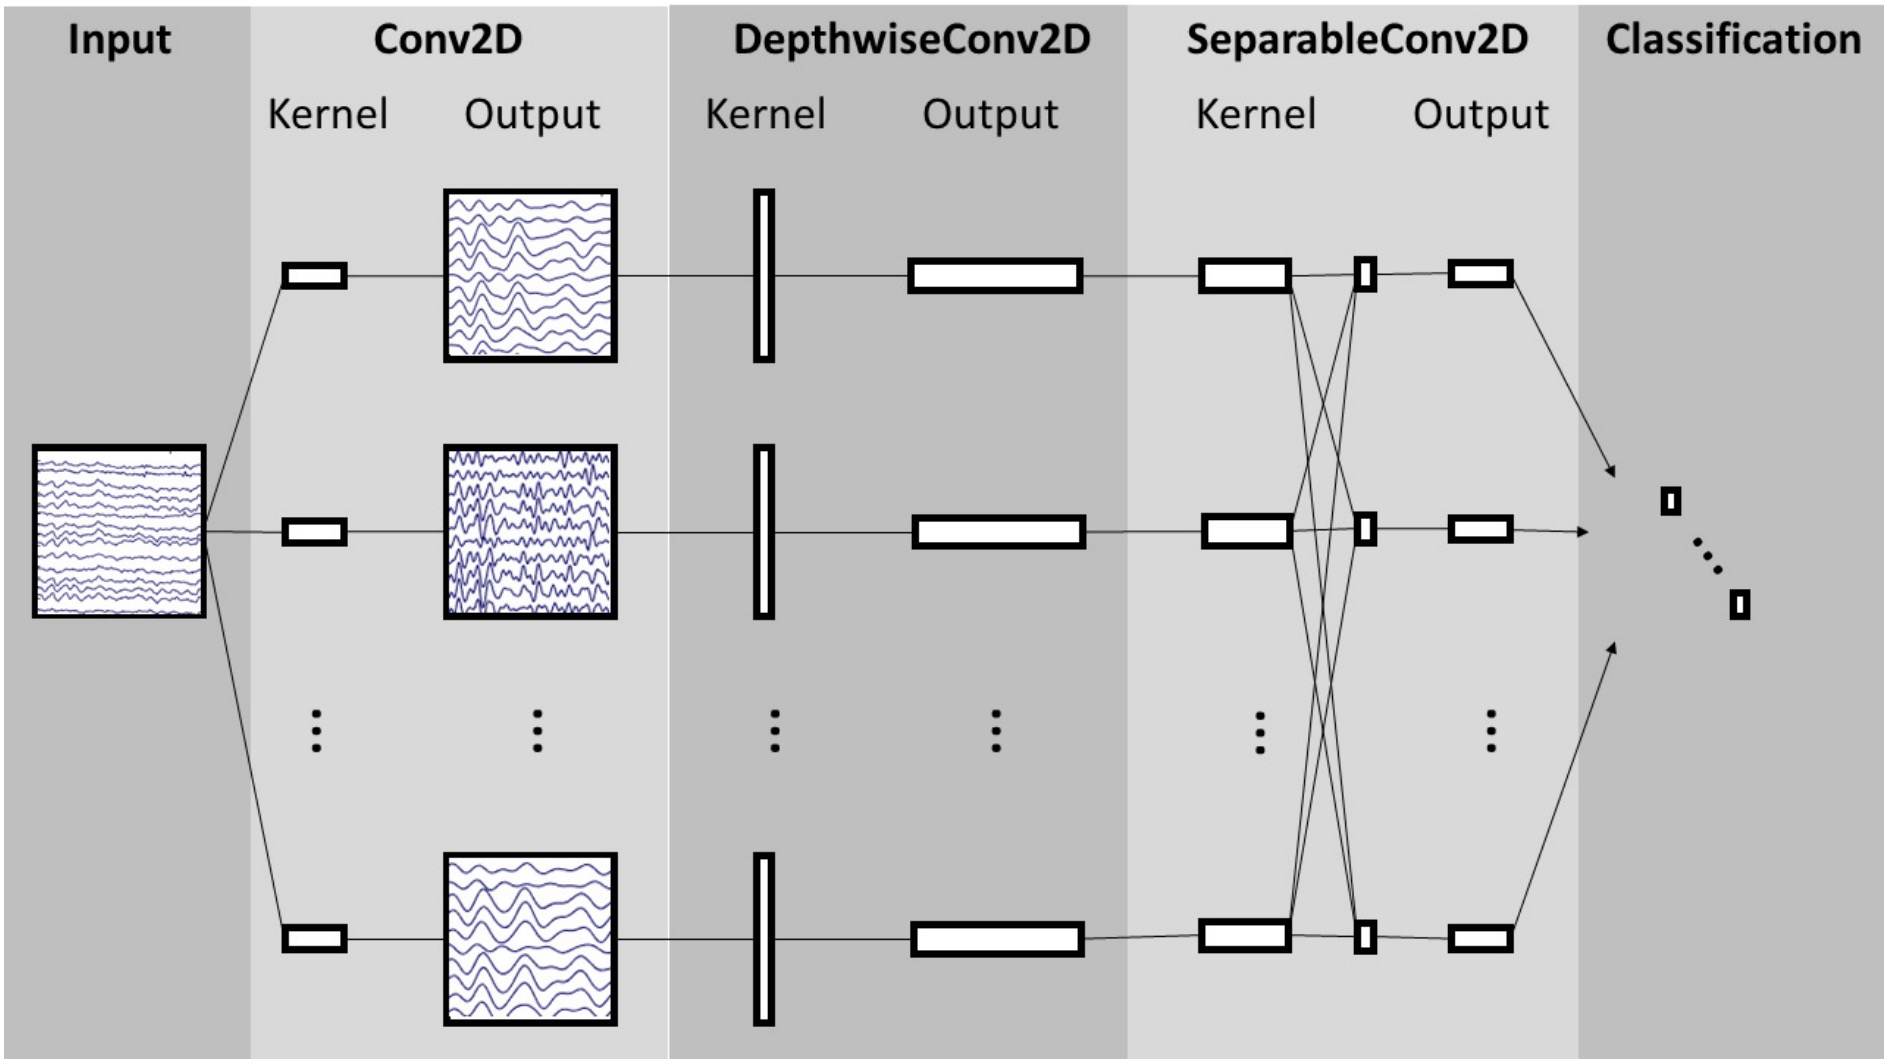
\includegraphics[width=0.7\textwidth]{img/EEGNet.jpg}
  \caption{EEGNet structure \cite{EEGNet}}
  \label{fig:EEGNet}
\end{figure}



\section{Results and Conclusion}


In conclusion, our efforts primarily revolved around gaining a comprehensive understanding of the dataset, including its construction, recording process, sampling techniques, and various parameters. With this understanding of the data, we set out to implement the EEGnet model in order to identify pathologies within individual epochs of EEG signals. Our initial findings indicated that the model was already performing well; however, we were able to significantly enhance its performance by transitioning from the ELU activation function to ReLU.

It is worth noting that the statistical population of the dataset was relatively small and not ideally suited for our specific task. To further refine the accuracy and robustness of our model, a more extensive and diverse dataset is imperative. While a larger volume of data per patient may not be necessary, a greater number of patients are indeed needed for comprehensive and reliable results.

As we look toward future endeavors for this project, it is crucial to ensure that our model is learning to identify diseases rather than individual patients. To achieve this, an idea is partitioning the dataset into distinct training and testing subsets, where the testing subset comprises patients who have never been encountered by the network during training. This approach will help mitigate the risk of overfitting to individual patients and advance the generalizability of our disease identification model.


\bibliographystyle{apalike}
\bibliography{references}

\end{document}